%% Does a Bankruptcy Model Trained in Calm Times Survive a Recession?
%% Single-column research manuscript.
\documentclass[manuscript,nonacm]{acmart}
\usepackage{paperstyle}

\graphicspath{{figures/}}

%% The template numbers its references, so override acmart's author-year default.
\citestyle{acmnumeric}

\begin{document}

\title{Does a Bankruptcy Model Trained in Calm Times Survive a Recession?}
\subtitle{A Temporal Stress Test on U.S. Public Firms}

\author{Ayush Bodalia}
\equalcontrib
\affiliation{%
  \institution{Nexus Labs}
  \country{USA}}

\author{Arnav Deokule}
\equalcontribmark
\affiliation{%
  \institution{Nexus Labs}
  \country{USA}}

\author{Shravan Ginde}
\equalcontribmark
\affiliation{%
  \institution{Nexus Labs}
  \country{USA}}

\author{Sahasra Namburu}
\equalcontribmark
\affiliation{%
  \institution{Nexus Labs}
  \country{USA}}

\author{Kavindran Rajangam}
\equalcontribmark
\affiliation{%
  \institution{Nexus Labs}
  \country{USA}}

\author{Sreehaas Voruganti}
\equalcontribmark
\affiliation{%
  \institution{Nexus Labs}
  \country{USA}}

\author{Srikanth Samy}
\affiliation{%
  \institution{University of California, Berkeley}
  \city{Berkeley}
  \state{California}
  \country{USA}}
\email{ssamy@berkeley.edu}

\author{Ishaan Gupta}
\affiliation{%
  \institution{Stanford University}
  \city{Stanford}
  \state{California}
  \country{USA}}
\email{ishaangupta@stanford.edu}

\begin{abstract}
Corporate-distress models are typically trained and validated on data pooled across
time, yet they are deployed forward into economic conditions that may differ sharply
from the training period. We ask whether a bankruptcy classifier trained on \emph{calm}
pre-crisis years still functions during a \emph{recession}. Using $78{,}682$
company-years of U.S. public firms (1999--2018) with $18$ financial variables, we frame
imminent-failure prediction---a firm's final reporting year before delisting---and
engineer $15$ Altman-style financial ratios. Training on 1999--2006 with a
company-grouped split to prevent leakage, a random forest attains a held-out ROC-AUC of
$0.755$, well ahead of logistic regression ($0.646$) and a multilayer perceptron
($0.625$); the distress boundary is strongly nonlinear. Stress-testing the frozen
calm-era models on the 2008--2009 recession, the random forest does not degrade but
\emph{improves} to $0.798$ AUC, while the linear and neural models slip. The
financial-distress signal is thus stable, even sharper, under crisis conditions: the
model survives the stress test. We also show that a naive per-year AUC curve suggests a
spurious ``cliff'' at 2007 that is an evaluation artifact of training-set overlap,
underscoring the importance of leakage-free temporal validation.
\end{abstract}

\ccsdesc[500]{Applied computing~Economics}
\ccsdesc[300]{Computing methodologies~Supervised learning by classification}
\ccsdesc[300]{Computing methodologies~Machine learning}

\keywords{bankruptcy prediction, distribution shift, temporal validation, financial
ratios, class imbalance}

\maketitle

\section{Introduction}
Models that flag firms at risk of failure are central to credit and investment
decisions. Their operational value depends on \emph{temporal} robustness: a model fit on
historical data must keep working as macroeconomic conditions evolve. The 2008 financial
crisis is a natural stress test---a sharp regime change between the calm mid-2000s and
the recession. We pose a direct question: \emph{does a distress model trained on calm
years still rank failing firms during the recession, and which model family is most
robust?}

Our contributions are: (i) an imminent-failure formulation of the widely used U.S.
bankruptcy dataset with leakage-controlled, company-grouped validation; (ii) a calm-era
baseline in which a random forest clearly outperforms linear and neural models; (iii) a
temporal stress test showing the random forest survives---indeed improves---on
2008--2009; and (iv) a cautionary analysis of a per-year evaluation artifact that can
masquerade as crisis-induced failure.

\section{Related Work}
Distress prediction dates to Beaver's univariate ratio analysis~\cite{beaver1966},
Altman's $Z$-score~\cite{altman1968}, and Ohlson's logit model~\cite{ohlson1980}, whose
ratio families we adopt. Hazard formulations that respect the panel structure of firm
data followed~\cite{shumway2001,campbell2008}. Machine-learning approaches, including
random forests~\cite{breiman2001}, are now standard, and tree ensembles remain strong on
tabular problems of this shape~\cite{grinsztajn2022}. The robustness of predictive
models under temporal or covariate shift is the subject of the dataset-shift
literature~\cite{quinonero2009}, and the specific failure mode we document in
\cref{sec:artifact} belongs to the literature on leakage in applied machine
learning~\cite{kaufman2012leakage,kapoor2023leakage}. We combine these threads into an
explicit calm-to-recession transfer evaluation on a large panel of U.S. firms.

\section{Data}
We use a public dataset of $78{,}682$ company-years for U.S. public companies,
1999--2018, each with $18$ accounting variables (assets, liabilities, income-statement
items, market value) and an \texttt{alive}/\texttt{failed} status. Failure is rare, so
plain accuracy is uninformative and we evaluate with ranking and precision--recall
metrics (\cref{fig:balance}). Distressed firms differ systematically from healthy
ones---lower profitability and higher leverage---which is the signal our models exploit.

\begin{figure}[t]
\centering
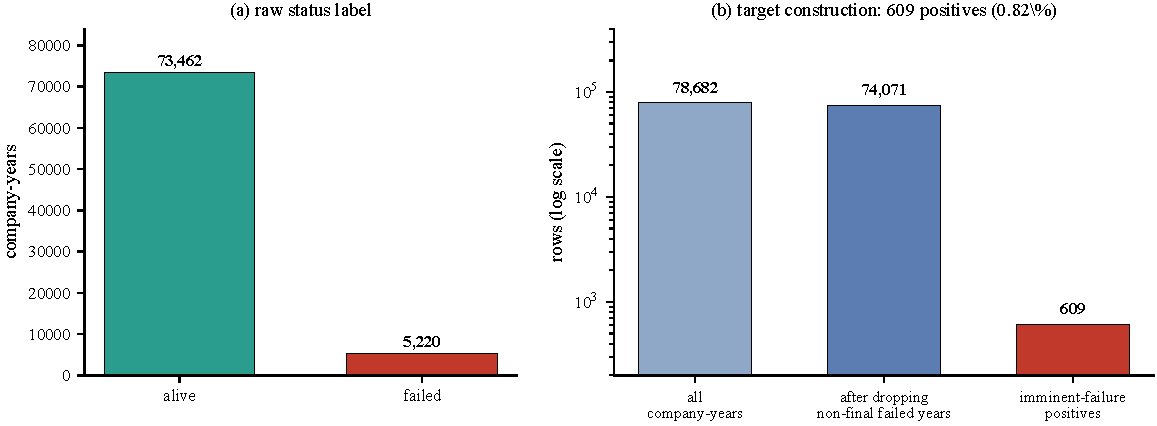
\includegraphics[width=\linewidth]{fig1_class_balance.pdf}
\caption{(a) Raw status labels: $6.6\%$ of company-years belong to firms that eventually
failed. (b) The imminent-failure target is far rarer still. Dropping the non-final years
of failed firms leaves $74{,}071$ rows, of which only $609$ ($0.82\%$) are positive.}
\label{fig:balance}
\end{figure}

\subsection{Target definition}
A failed firm appears in the panel for several years, every one of them stamped
\texttt{failed}. Labelling all of those years as bankruptcies would be misleading,
because a firm five years from delisting usually looks healthy. We therefore label a
company-year positive if and only if it is that firm's \emph{final} reporting year,
\begin{equation}
y_{it}=\ind\!\left[\text{status}_i=\texttt{failed}\ \wedge\
                    t=\max\{t': (i,t')\in\mathcal{D}\}\right],
\label{eq:target}
\end{equation}
and we drop the earlier years of failed firms so that the negative class is clean. This
yields $609$ positives among $74{,}071$ company-years, a base rate of $0.82\%$. The
label is a proxy: a firm's last filing is not always the year it legally enters
bankruptcy.

\subsection{Features}
Raw dollar magnitudes are size-confounded---a \$1M loss is fatal for a small firm and a
rounding error for a large one. From the $18$ raw variables we therefore build $15$
Altman-style ratios~\cite{altman1968,ohlson1980}: return on assets, EBIT/assets,
EBITDA/assets, working-capital/assets, retained-earnings/assets, sales/assets, leverage,
long-term-debt/assets, market-value/liabilities, current ratio, gross and net margins,
inventory/assets, receivables/assets, and $\log(1+\text{total assets})$ as a size term.
Each is winsorized at the training-set $1$st and $99$th percentiles, median-imputed, and
standardized, with all three statistics estimated on the training rows only:
\begin{equation}
\tilde{x}_{j}=\frac{\operatorname{clip}\!\left(x_{j};\,q^{\text{tr}}_{0.01,j},\,q^{\text{tr}}_{0.99,j}\right)-\mu^{\text{tr}}_{j}}{\sigma^{\text{tr}}_{j}} .
\label{eq:preproc}
\end{equation}

\section{Methods}

\subsection{Models and metrics}
Logistic regression predicts $\hat{p}(x)=\sigma(w^{\!\top}\tilde{x}+b)$; the random
forest~\cite{breiman2001} averages $400$ decision trees with a minimum of three samples
per leaf; the MLP applies two ReLU hidden layers ($64$ and $32$ units) with dropout
$0.3$ and a sigmoid output, trained with Adam~\cite{kingma2015adam} and early stopping.
Given the extreme imbalance, all models use class weighting; the MLP minimizes a
weighted binary cross-entropy
\begin{equation}
\mathcal{L}=-\frac{1}{N}\sum_{i=1}^{N}
  \left[\beta_1 y_i\log\hat{y}_i+\beta_0(1-y_i)\log(1-\hat{y}_i)\right],
\qquad \beta_c=\frac{N}{2N_c}.
\label{eq:loss}
\end{equation}
We report ROC-AUC, the probability that a failing firm is ranked above a surviving
one~\cite{fawcett2006},
\begin{equation}
\mathrm{AUC}=\Pr\!\left(\hat{p}(x^{+})>\hat{p}(x^{-})\right),
\label{eq:auc}
\end{equation}
and PR-AUC (average precision), whose no-skill baseline equals the positive rate. With a
base rate near $0.6\%$, PR-AUC is the more demanding summary and the more honest one for
a rare-event problem~\cite{davis2006,saito2015}.

\subsection{Validation protocol}
The calm era (1999--2006) is split \emph{by company} using a grouped shuffle split, so
that a firm never appears in both training and calm-test partitions. This matters
because each firm contributes several highly correlated yearly rows; a random row split
would let the model recognise a company rather than learn a warning sign. The recession
window (2008--2009) is held out entirely for the stress test, and 2007 is excluded as a
transition year. \cref{fig:splits} summarises the resulting partitions.

\begin{figure}[t]
\centering
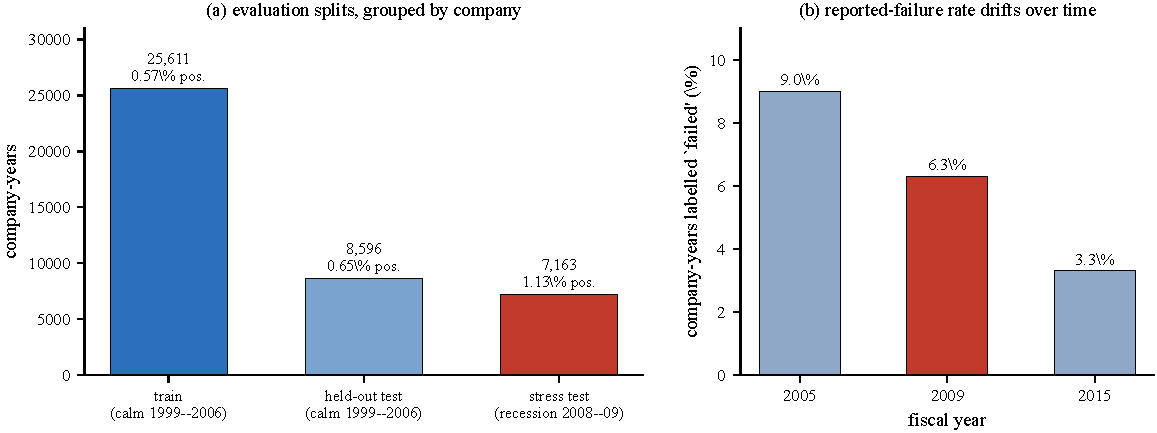
\includegraphics[width=\linewidth]{fig2_splits.pdf}
\caption{(a) The three evaluation partitions, with sizes and positive rates. The
recession window carries roughly twice the imminent-failure rate of the calm training
data ($1.13\%$ versus $0.57\%$). (b) The share of company-years labelled
\texttt{failed} drifts substantially over the panel.}
\label{fig:splits}
\end{figure}

We define the calm-to-recession \emph{change} as
\begin{equation}
\Delta=\mathrm{AUC}_{\text{recession}}-\mathrm{AUC}_{\text{calm}},
\label{eq:change}
\end{equation}
where both terms are computed on firms excluded from training. A non-negative $\Delta$
means the model survives the regime shift.

\section{Experiments and Results}

\subsection{Calm-era baseline}
\cref{tab:calm} reports held-out calm-era performance. The random forest ($0.755$ AUC)
clearly beats logistic regression ($0.646$) and the MLP ($0.625$): the mapping from
financial ratios to imminent failure is strongly nonlinear and interaction-heavy---low
profitability \emph{and} high leverage \emph{and} weak liquidity---which the tree
ensemble captures and the linear and shallow models do not. PR-AUC is low throughout, an
honest consequence of the $\sim\!0.6\%$ base rate; even so, the random forest's $0.020$
is roughly $3\times$ the no-skill baseline.

\begin{table}[t]
\centering
\caption{Held-out calm-era (1999--2006) performance, company-grouped split. The PR-AUC
no-skill baseline is the positive rate, $0.0065$.}
\label{tab:calm}
\begin{tabular}{lrr}
\toprule
Model & ROC-AUC & PR-AUC\\
\midrule
Logistic Regression & 0.646 & 0.010\\
Random Forest       & \textbf{0.755} & \textbf{0.020}\\
MLP                 & 0.625 & 0.012\\
\bottomrule
\end{tabular}
\end{table}

\subsection{The 2008--2009 stress test}
\cref{tab:stress} and \cref{fig:stress} report the frozen calm-era models applied to the
recession. The random forest does not degrade; its AUC \emph{rises} to $0.798$
($\Delta=+0.042$). The linear and neural models slip modestly ($\Delta=-0.031$ and
$-0.050$). Firms about to fail during the crisis are, if anything, \emph{easier} to
identify from their financial ratios than in calm times---distress is a stable, even
sharpened, signal. By ranking, the model survives the stress test.

\begin{table}[t]
\centering
\caption{Calm-era versus 2008--2009 recession, both on firms excluded from training.
$\Delta$ is defined in Eq.~\eqref{eq:change}.}
\label{tab:stress}
\begin{tabular}{lrrr}
\toprule
Model & Calm AUC & Recession AUC & $\Delta$\\
\midrule
Logistic Regression & 0.646 & 0.615 & $-0.031$\\
Random Forest       & 0.755 & \textbf{0.798} & $\bm{+0.042}$\\
MLP                 & 0.625 & 0.575 & $-0.050$\\
\bottomrule
\end{tabular}
\end{table}

\begin{figure}[t]
\centering
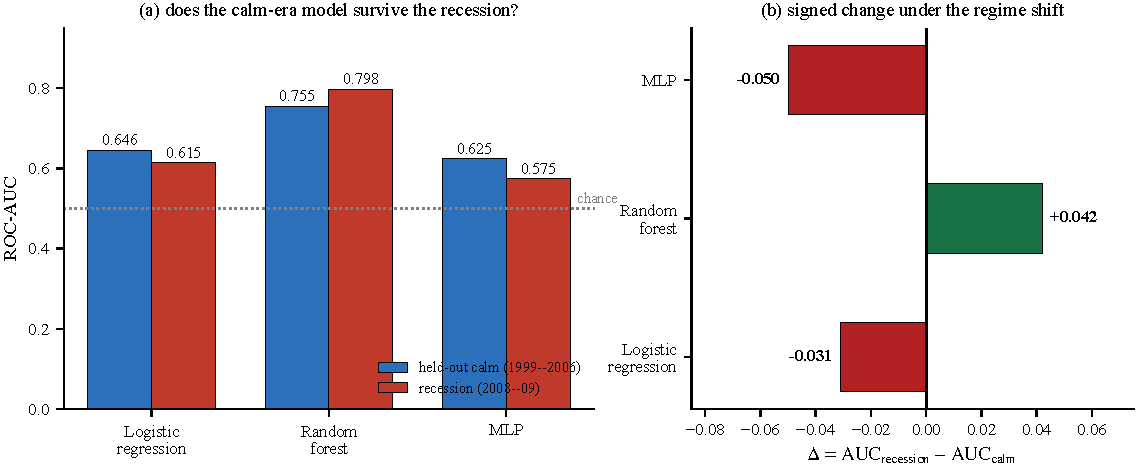
\includegraphics[width=\linewidth]{fig3_stress_test.pdf}
\caption{(a) Calm versus recession ROC-AUC per model. Taller red than blue means the
model holds up. (b) The signed change of Eq.~\eqref{eq:change}: only the random forest
is positive, and it is the only model that was strong to begin with.}
\label{fig:stress}
\end{figure}

Two points qualify the headline. First, the recession's higher base rate ($1.13\%$
versus $0.57\%$) raises the attainable precision independently of model quality, so part
of the PR-AUC improvement is mechanical rather than evidence of better discrimination;
this is why we make ROC-AUC the primary endpoint. Second, the ranking that survives is
not a calibrated probability. A threshold tuned on calm-era scores will fire at a
different rate when the underlying failure rate roughly doubles, so operating points
must be re-calibrated even though the ordering is preserved~\cite{vancalster2019}.

\subsection{A per-year artifact that looks like a crisis break}
\label{sec:artifact}
It is natural to diagnose temporal robustness by scoring the calm-trained model on every
fiscal year and plotting the resulting AUC curve. Doing so produces an apparent
``cliff'' after 2006 that invites the reading that the crisis broke the model. It is
largely an evaluation artifact.

The mechanism is straightforward. Pre-2007 years still contain many of the exact firms
the model trained on, and because a firm's yearly rows are highly correlated, scoring
those years measures partial memorisation rather than prediction. Later years contain
genuinely unseen firms. The apparent drop is therefore not the crisis arriving; it is
the evaluation finally becoming honest. This is a textbook instance of the leakage
patterns catalogued in~\cite{kaufman2012leakage,kapoor2023leakage}: the contaminated
estimate is not merely optimistic, it induces a qualitatively wrong conclusion about
\emph{when} performance changed.

The leakage-free comparison shows no break at all. \cref{fig:artifact} places the two
valid estimates side by side: held-out calm firms at $0.755$ and held-out recession
firms at $0.798$. The correct reading of the same underlying model is that performance
rose across the regime change.

\begin{figure}[t]
\centering
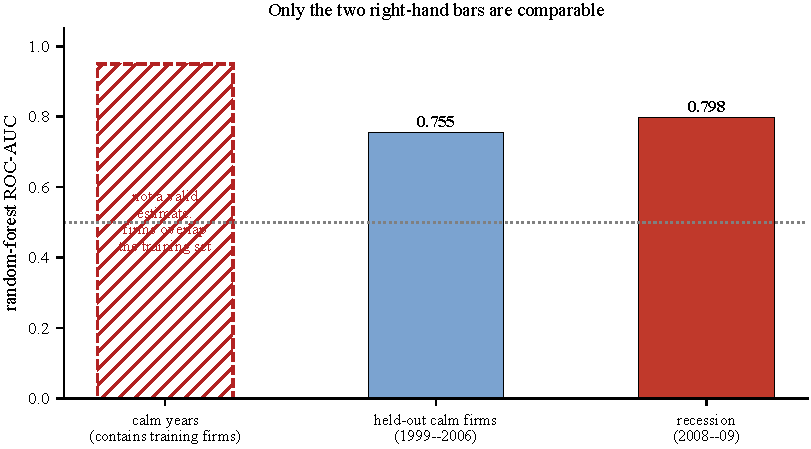
\includegraphics[width=0.72\linewidth]{fig4_leakage_artifact.pdf}
\caption{Only estimates computed on firms excluded from training are comparable. A
per-year curve scored on calm years is contaminated by training-firm overlap (left,
hatched) and cannot be placed on the same axis as the two valid estimates.}
\label{fig:artifact}
\end{figure}

The practical rule follows directly: in panel data, temporal validation must exclude a
firm's \emph{entire} history from the test period, not merely the test year.

\section{Discussion}
The headline is reassuring and slightly counterintuitive: a distress model built before
the crisis survives the crisis, and the most flexible model is also the most robust.
Because financial ratios encode the mechanics of insolvency---eroding profitability,
mounting leverage, shrinking liquidity---the calm-era decision surface transfers to the
recession, where these signatures are sharper.

That the random forest is simultaneously the most accurate and the most robust deserves
comment, because flexibility and robustness are often assumed to trade off. Here the
distress boundary is genuinely nonlinear, so the linear model is misspecified in both
regimes and has no robustness advantage to offer; its smaller absolute loss under shift
comes with a much lower absolute score. The MLP, fitting $\sim\!150$ positives, is
data-starved rather than over-flexible. The practical caveats concern calibration and
measurement, not ranking.

\section{Limitations}
Positives are rare, so PR-AUC is low and the recession estimates rest on a few dozen
failures; they should be read as directional. The imminent-failure label---the final
reporting year---is a proxy for the legal bankruptcy date. Firms recur across the calm
and recession windows, so the transfer is across \emph{time} rather than to entirely new
firms; this is realistic for re-scoring a portfolio but is a caveat for generalization
to unseen issuers. We report a single seed and a single design, with no confidence
intervals, so differences smaller than roughly $0.02$ AUC should not be interpreted.
Finally, survivorship and reporting biases affect which firms appear in the panel at all.

\section{Conclusion}
On a large panel of U.S. public firms, a random forest trained on calm pre-crisis years
predicts imminent bankruptcy at $0.755$ ROC-AUC and \emph{survives} the 2008--2009
recession, improving to $0.798$, while simpler models slip. Financial-distress signals
are temporally robust, and a per-year evaluation artifact can falsely suggest a
crisis-induced collapse. We recommend leakage-free temporal validation and threshold
re-calibration for deployment across economic regimes.

\section*{Reproducibility}
The analysis notebook fixes all random seeds, defines the target and the
company-grouped split explicitly, and estimates every preprocessing statistic inside the
training partition. The source panel is licensed and is not redistributed here; the
figure script accompanying this manuscript regenerates all figures and tables from the
recorded results, and recomputes the per-year analysis when the raw CSV is supplied.

\bibliographystyle{ACM-Reference-Format}
\bibliography{refs}

\section*{Authors' background}

\noindent\begin{minipage}{\linewidth}
\begin{tabular}{@{}p{0.24\linewidth}p{0.18\linewidth}p{0.22\linewidth}p{0.22\linewidth}@{}}
\toprule
Your Name & Title$^{*}$ & Research Field & Personal website \\
\midrule
Ayush Bodalia      & & & \\
Arnav Deokule      & & & \\
Shravan Ginde      & & & \\
Sahasra Namburu    & & & \\
Kavindran Rajangam & & & \\
Sreehaas Voruganti & & & \\
Srikanth Samy      & & & \\
Ishaan Gupta       & & & \\
\bottomrule
\end{tabular}

\vskip 6pt
{\footnotesize $^{*}$This form helps us to understand your paper better,
the form itself will not be published.\\
$^{*}$Title can be chosen from: master student, Phd candidate, assistant professor,
lecture, senior lecture, associate professor, full professor}
\end{minipage}

\end{document}
